\subsection{问题三的模型建立与求解}

问题三将前两问扩展为由模拟器反馈驱动的连续决策过程，包括八点扫描、观测更新、批量补充定位、
清除路线排序和逐源清除。

\subsubsection{执行状态与行动时间}

记当前位置、检测频道和累计虚拟时间为 $p,h,t$；频道集合分为已发现未清除、无源和已清除三类
$\mathcal C_f,\mathcal C_a,\mathcal C_c$。每个已发现频道保存区域 $\widehat K_j$、最小包围圆
$(c_j,r_j)$ 和清除队列 $Q_j$ 等状态。

机器狗每次只发出进入、检测、清除或退出中的一个动作，收到并处理该动作的响应后才生成下一动作。设机器狗从 $p$ 移动到 $s$，速度为 $v=5\ \mathrm{m/s}$，换频时间为 $\tau_{\mathrm{sw}}=1\ \mathrm{s}$，检测时间为 $\tau_{\mathrm{meas}}=5\ \mathrm{s}$，则检测动作的虚拟时间为
\begin{equation}
  T_{\mathrm{measure}}(p,h;s,j)
  =\frac{\|s-p\|_2}{v}
  +\tau_{\mathrm{sw}}\mathbf 1_{\{h\ne j\}}
  +\tau_{\mathrm{meas}}.
  \label{eq:q3-measure-time}
\end{equation}

若在 $s$ 对频道 $j$ 执行清除，光电操作耗时 $3\ \mathrm{s}$，清除成功时激光发射再耗时 $2\ \mathrm{s}$。记清除结果为 $b\in\{0,1\}$，其中 $b=1$ 表示成功，则
\begin{equation}
  T_{\mathrm{clear}}(p;s,b)
  =\frac{\|s-p\|_2}{v}+3+2b.
  \label{eq:q3-clear-time}
\end{equation}

两式用于后续选点与排序，现实计算时间不计入虚拟行动时间。

\subsubsection{八个等角驻留点的初始扫描}

记目标分布区域为 $\mathcal D=\overline B(O_0,1800)$。

由于每个全向干扰源的有效接收半径至少为 $1000\ \mathrm{m}$，只要扫描驻留点集合对 $\mathcal D$ 的覆盖半径不超过 $1000\ \mathrm{m}$，就能保证每个源至少在一个驻留点被发现。本文取环半径 $a=960\ \mathrm{m}$，在圆周上设置八个等角驻留点
\begin{equation}
  P_k=O_0+a
  \left(\cos\frac{k\pi}{4},\sin\frac{k\pi}{4}\right),
  \qquad k=0,1,\ldots,7.
  \label{eq:q3-eight-points}
\end{equation}

机器狗从原点依次访问 $P_0,\ldots,P_7$，在每点先检测当前频道，再检测其他频道。
布局、顺序及保证接收圆如图~\ref{fig:q3-eight-point-scan} 所示。

\begin{figure}[H]
  \centering
  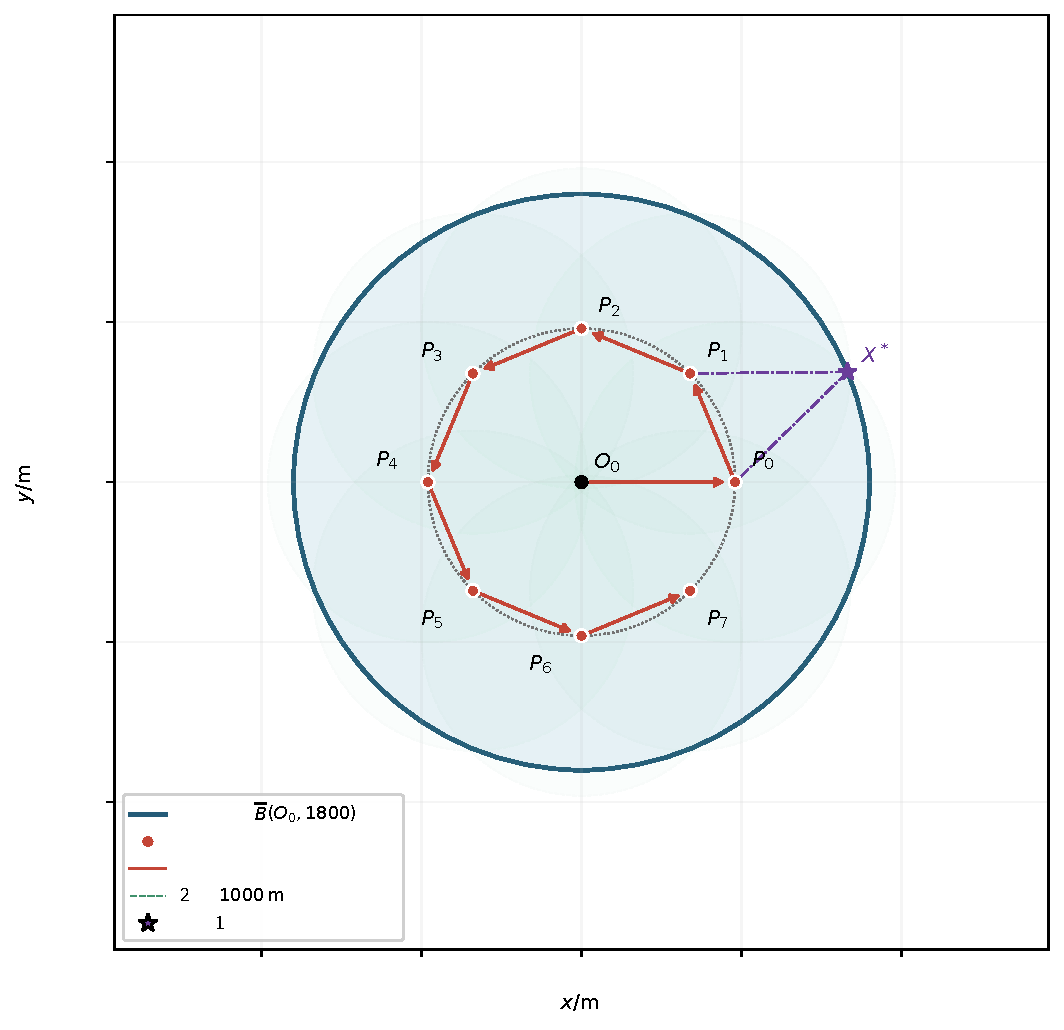
\includegraphics[width=0.78\textwidth]{figures/q3-eight-point-scan.pdf}
  \caption{八点扫描及保证接收覆盖：箭头表示访问顺序，$X^*$ 为最不利边界位置}
  \label{fig:q3-eight-point-scan}
\end{figure}

\noindent\textbf{命题 3：}{\kaishu 式~\eqref{eq:q3-eight-points} 给出的八个驻留点能够以小于 $1000\ \mathrm{m}$ 的覆盖半径覆盖整个目标圆形区域 $\mathcal D$。}

\noindent\textbf{证明：}
任取 $X\in\mathcal D$，以 $O_0$ 为极点写成极坐标 $(\rho,\theta)$，其中 $0\leq\rho\leq1800$。八个驻留点将圆周方向等分，因此必存在某个 $P_k$，使 $X$ 与 $P_k$ 的极角差 $\Delta$ 满足 $|\Delta|\leq\pi/8$。由余弦定理，
\begin{equation}
  \|X-P_k\|_2^2
  =\rho^2+a^2-2a\rho\cos\Delta.
  \label{eq:q3-cover-distance}
\end{equation}

该式对 $\rho$ 为凸函数，并随 $|\Delta|$ 增大，故只需比较圆心与目标圆周角平分方向。代入 $a=960$ 得
\begin{equation}
  \begin{aligned}
    d_{\mathrm{cov}}
    &=\max_{X\in\mathcal D}\min_{0\leq k\leq7}\|X-P_k\|_2,\\
    &=\max\left\{960,
      \sqrt{1800^2+960^2-2(1800)(960)\cos(\pi/8)}
      \right\},\\
    &\approx984.212\ \mathrm{m}<1000\ \mathrm{m}.
  \end{aligned}
\end{equation}

故八点布局覆盖整个目标区域。\hfill$\square$

近距离结果立即原地清除；有效示向度用于更新区域；无信号时继续扫描。

设频道 $j$ 已在位置 $S_{j,1},\ldots,S_{j,m}$ 获得示向度 $\theta_{j,1},\ldots,\theta_{j,m}$。沿用问题一的角度误差半平面交，并加入问题二的目标圆形区域与接收距离上界，实时计算使用的源位置外近似为
\begin{equation}
  \widehat K_j^{(m)}
  =\widehat B_{\mathrm{out}}^{(N_3)}(O_0,1800)
  \cap\bigcap_{i=1}^{m}
  \left[
  C(S_{j,i},\theta_{j,i},\varepsilon)
  \cap\widehat B_{\mathrm{out}}^{(N_3)}(S_{j,i},1500)
  \right],
  \qquad N_3=16.
  \label{eq:q3-region-update}
\end{equation}

其中 $\varepsilon=1.005^\circ$，实时圆盘外切多边形边数 $N_3=16$。
$\widehat K_j^{(m)}$ 是包含真实源的有界凸多边形，且新增观测只会加入约束，因此
\begin{equation}
  \widehat K_j^{(m+1)}\subseteq\widehat K_j^{(m)}.
  \label{eq:q3-nested-regions}
\end{equation}

随后计算 $\widehat K_j^{(m)}$ 的最小包围圆
\begin{equation}
  \widehat K_j^{(m)}\subseteq\overline B(c_j,r_j),
  \qquad r_j=\rho\bigl(\widehat K_j^{(m)}\bigr).
  \label{eq:q3-mec}
\end{equation}

对扫描中已经发现的频道，记候选扫描点 $P_k$ 相对当前区域中心与已有第 $i$ 个检测点形成的夹角为
\begin{equation}
  \alpha_{j,i}(P_k)
  =\angle\bigl(c_j-S_{j,i},c_j-P_k\bigr),
  \qquad
  \alpha_j(P_k)=\max_i\alpha_{j,i}(P_k).
\end{equation}

若 $r_j\leq15\ \mathrm{m}$ 或 $\alpha_j(P_k)<30^\circ$，则跳过重复检测；否则顺路补充示向度。
该规则只减少低价值检测，不作为最优性结论。

由扫描覆盖结论，八点扫描后仍未发现的频道可归入 $\mathcal C_a$；已发现未清除及已清除频道分别归入 $\mathcal C_f,\mathcal C_c$。三类互不相交，合起来包含全部 $20$ 个频道。

\subsubsection{批量补充定位与停止规则}

扫描阶段结束后，暂不立即逐个往返清除，而是先把所有已发现源处理成有限清除队列。设当前尚未入队的频道集合为 $\mathcal U$，策略按
\begin{equation}
  j^*=\operatorname*{arg\,min}_{j\in\mathcal U}\|p-c_j\|_2
  \label{eq:q3-nearest-source}
\end{equation}

选取距当前位置最近的源作为暂定的下一处理对象。

按定位半径处理：$r_{j^*}\leq19.9\ \mathrm m$ 时将中心加入可靠清除队列；
$19.9<r_{j^*}\leq40\ \mathrm m$ 时加入中心及保底清除点；$r_{j^*}>40\ \mathrm m$ 且补充次数
小于 $M=2$ 时选择新检测点。

补充检测沿用问题二，并按真实响应更新区域；每源最多两次。达到上限后转入有限保底清除队列。
$40\ \mathrm{m}$ 只表示可先试中心并继续保底点，不是中心可靠清除条件。

\subsubsection{开放式旅行商清除顺序}

所有已发现源均形成清除队列后，取各队列的首点，即最小包围圆中心 $c_1,\ldots,c_n$，建立完全图，边权为欧氏距离
\begin{equation}
  d_{ij}=\|c_i-c_j\|_2.
\end{equation}

清除结束后无需返回起点，因此采用开放式旅行商路径而非闭合回路。程序使用 Held--Karp 动态规划的开放式变体求中心之间的最短访问顺序~\cite{heldkarp1962}。对任意非空中心下标集合 $A\subseteq\{1,\ldots,n\}$ 及 $j\in A$，定义
\begin{equation}
  F(A,j)=\text{恰好访问 $A$ 中全部中心且以 $c_j$ 结束的最短内部路径长度}.
\end{equation}

因为路径起点可取 $A$ 中任一中心，初值和递推式为
\begin{equation}
  F(\{j\},j)=0,
  \qquad
  F(A,j)=\min_{i\in A\setminus\{j\}}
  \left[F(A\setminus\{j\},i)+d_{ij}\right].
  \label{eq:q3-held-karp}
\end{equation}

最终中心内部路径长度为
\begin{equation}
  L_{\mathrm{TSP}}
  =\min_{1\leq j\leq n}F(\{1,\ldots,n\},j),
  \label{eq:q3-open-tsp}
\end{equation}

并通过保存的前驱状态回溯得到访问次序。

递推利用最短路径的最优子结构~\cite{heldkarp1962}，时间、空间复杂度分别为
$O(n^2 2^n)$ 和 $O(n2^n)$，适用于 $n\leq16$。它只优化中心之间的内部路径，
不代表整个搜索、定位和清除过程全局最优。

图~\ref{fig:q3-clear-route} 给出一次日志回放中的实际清除路线。

\begin{figure}[H]
  \centering
  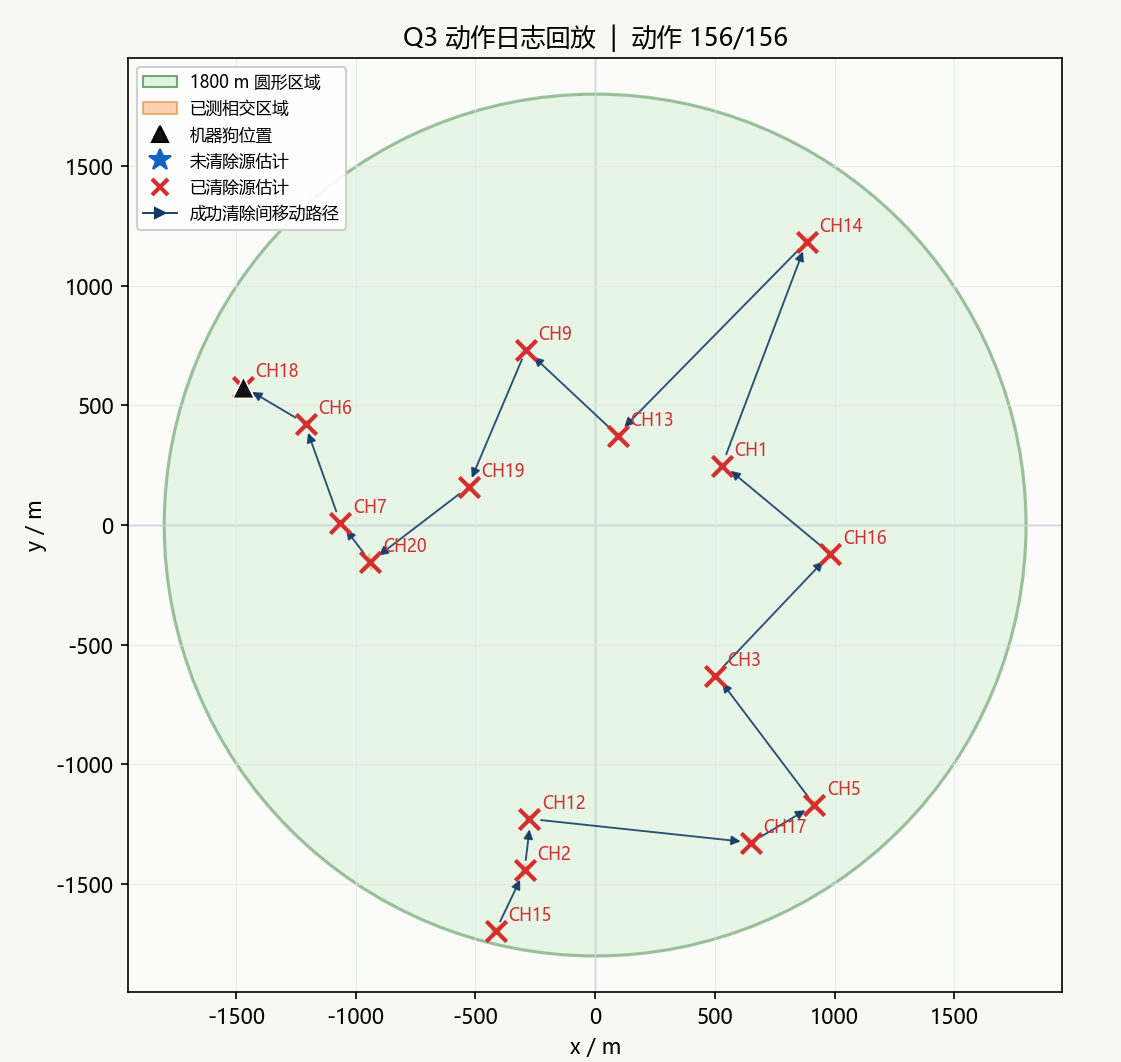
\includegraphics[width=0.72\textwidth]{figures/q3-route.png}
  \caption{问题三动作日志回放中的机器狗成功清除路线}
  \label{fig:q3-clear-route}
\end{figure}

\subsubsection{清除邻域偏移与保底覆盖}

按照开放式旅行商顺序清除已完成可靠定位的频道时，可以利用 $20\ \mathrm{m}$ 清除半径提前向下一目标移动。设当前源的最小包围圆为 $\overline B(c_j,r_j)$，下一队列中心为 $c_q$。当 $c_q\ne c_j$ 时，定义实际清除点
\begin{equation}
  y_j=c_j+(20-r_j)\frac{c_q-c_j}{\|c_q-c_j\|_2},
  \qquad r_j\leq19.9.
  \label{eq:q3-tspn-point}
\end{equation}

若当前源为最后一个源，或两中心重合，则取 $y_j=c_j$。

对任意真实源位置 $X_j\in\widehat K_j$，由三角不等式，
\begin{equation}
  \|X_j-y_j\|_2
  \leq\|X_j-c_j\|_2+\|c_j-y_j\|_2
  \leq r_j+(20-r_j)=20\ \mathrm m.
\end{equation}

因此偏移后仍能可靠清除，并沿下一目标方向前移 $20-r_j$ 米。

对尚未完成可靠定位的频道，策略先在 $c_j$ 试清除；失败后依次访问有限个保底清除点。为说明完整保底清除点构造，设 $k=\lceil r_j/20\rceil$，在中心放置一个保底清除点，并在第 $\ell$ 个同心圆上均匀放置 $6\ell$ 个保底清除点：
\begin{equation}
  q_{\ell,m}=c_j+20\ell
  \left(\cos\frac{2\pi m}{6\ell},
  \sin\frac{2\pi m}{6\ell}\right),
  \quad
  \ell=1,\ldots,k,\quad m=0,\ldots,6\ell-1.
  \label{eq:q3-probes}
\end{equation}

若某个保底清除点落在 $\widehat K_j$ 外，则将其投影到该凸多边形的最近点。完整保底清除点数量为
\begin{equation}
  N_{\mathrm{probe}}(k)=1+\sum_{\ell=1}^{k}6\ell
  =1+3k(k+1).
  \label{eq:q3-probe-count}
\end{equation}

\noindent\textbf{命题 4：}{\kaishu 式~\eqref{eq:q3-probes} 生成的不经过投影的保底清除点集合，以每个点 $20\ \mathrm{m}$ 的作用半径覆盖最小包围圆 $\overline B(c_j,r_j)$；将其中落在凸区域 $\widehat K_j$ 外的点投影到 $\widehat K_j$ 边界后，对 $\widehat K_j$ 内任意真实源位置的覆盖性质仍然成立。}

\noindent\textbf{证明：}
任取 $X\in\overline B(c_j,r_j)$。若 $\rho=\|X-c_j\|_2\leq10$，中心点即可覆盖；
否则取最近整数环号及该环上极角最近的点，则
$|\rho-20\ell|\leq10$、$|\Delta|\leq\pi/(6\ell)$。由余弦定理，
\begin{align}
  \|X-q_{\ell,m}\|_2^2
  &=(\rho-20\ell)^2+2\rho(20\ell)(1-\cos\Delta)\\
  &\leq100+\rho(20\ell)\frac{\pi^2}{36\ell^2}\\
  &\leq100+\frac{(20\ell+10)(20\ell)\pi^2}{36\ell^2}\\
  &\leq100+\frac{50\pi^2}{3}<400.
\end{align}

故存在距离小于 $20\ \mathrm m$ 的保底点。若 $q\notin\widehat K_j$，凸集投影满足
\begin{equation}
  \|X-\Pi_{\widehat K_j}(q)\|_2^2
  \leq\|X-q\|_2^2,
  \qquad X\in\widehat K_j,
\end{equation}

故投影不破坏覆盖。\hfill$\square$

每频道最多保留 $76$ 个保底点。当 $r_j\leq80\ \mathrm m$ 时完整点数至多为 $61$，覆盖保证保留；
$r_j>80\ \mathrm m$ 时队列会被截断，只能视为有限次尝试。

执行清除队列时，若当前点清除成功，则将频道加入 $\mathcal C_c$ 并转向下一队列；若失败，则删除当前队首并尝试下一个保底清除点。若所有频道最终满足
\begin{equation}
  \mathcal C_a\cup\mathcal C_c=\{1,2,\ldots,20\},
  \qquad \mathcal C_a\cap\mathcal C_c=\varnothing,
  \label{eq:q3-exit-condition}
\end{equation}

机器狗发出退出动作。在模拟器响应符合题设且保底分支满足 $r_j\leq80\ \mathrm m$ 时，
八点扫描、至多两次补充定位和有限清除队列保证策略在有限动作内完成。完整过程见
图~\ref{fig:q3-decision-tree}。

\begin{figure}[H]
  \centering
  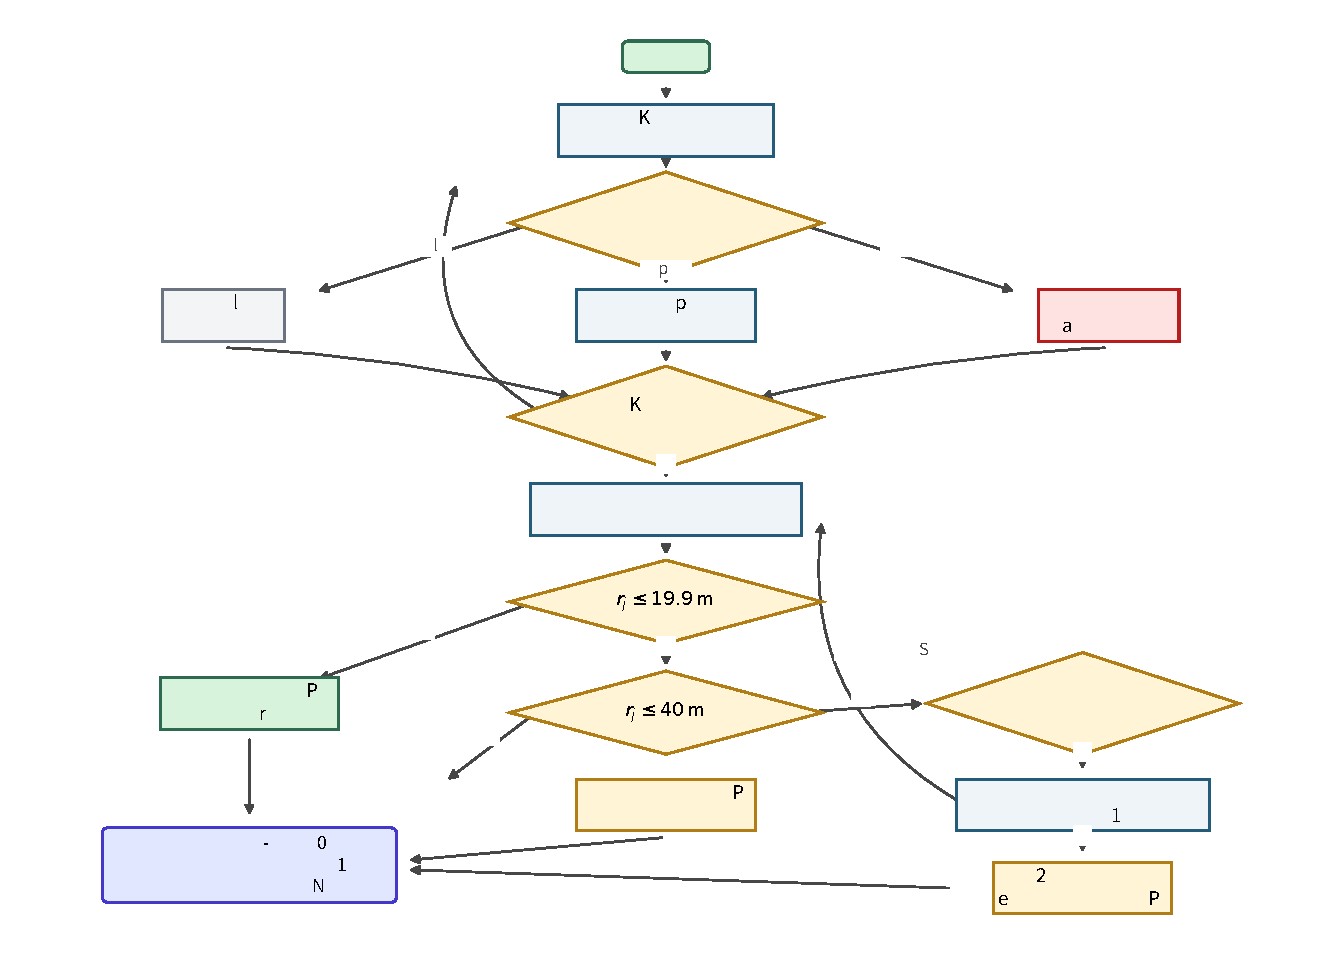
\includegraphics[width=0.98\textwidth]{figures/q3-decision-tree.pdf}
  \caption{问题三机器狗搜索、定位、路线排序与清除的决策树}
  \label{fig:q3-decision-tree}
\end{figure}
